\newpage
\section{Results}
\label{sec:results}




The asymptotic approximation~\cite{AsymptCLs} of the LHC
$\mathrm{CL_s}$ method~\cite{CLs1,CLs3} is used to set upper limits on
the cross sections for resonance production. The dominant sources of
systematic uncertainties are treated as nuisance parameters associated
with log-normal priors in those variables, following the methodology
described in Ref.~\cite{ATLASCMSstat}. For a given value of the
signal cross section, the nuisance parameters are fixed to the values
that maximize the likelihood, a method referred to as
profiling. The dependence of the likelihood on parameters used to
describe the background in Eq.~(\ref{eqParam}) is removed in the same
manner, and no additional systematic uncertainty is therefore assigned
to the parameterization of the background.

The HP and LP event categories are combined into a common likelihood,
with the two uncertainties in the $\PW/\cPZ$-tagging efficiencies
considered to be anticorrelated between HP and LP tagging because of
the exclusive selection on $\tau_{21}$, while the remaining systematic
uncertainties in signal are taken as fully correlated. The variables
describing the background uncertainties are treated as uncorrelated
between the two categories. The LP category contributes to the
sensitivity of the analysis, especially at large values of
$m_\mathrm{jj}$. The combined expected limits on the \GRS $\to\PW\PW$
production cross sections are, respectively, a factor of 1.1 and 1.6
smaller at $m_\mathrm{jj}=1.0$\TeVcc and 2.9\TeVcc than the limit
obtained from the HP category alone.


\begin{figure}[h!tb]
\centering
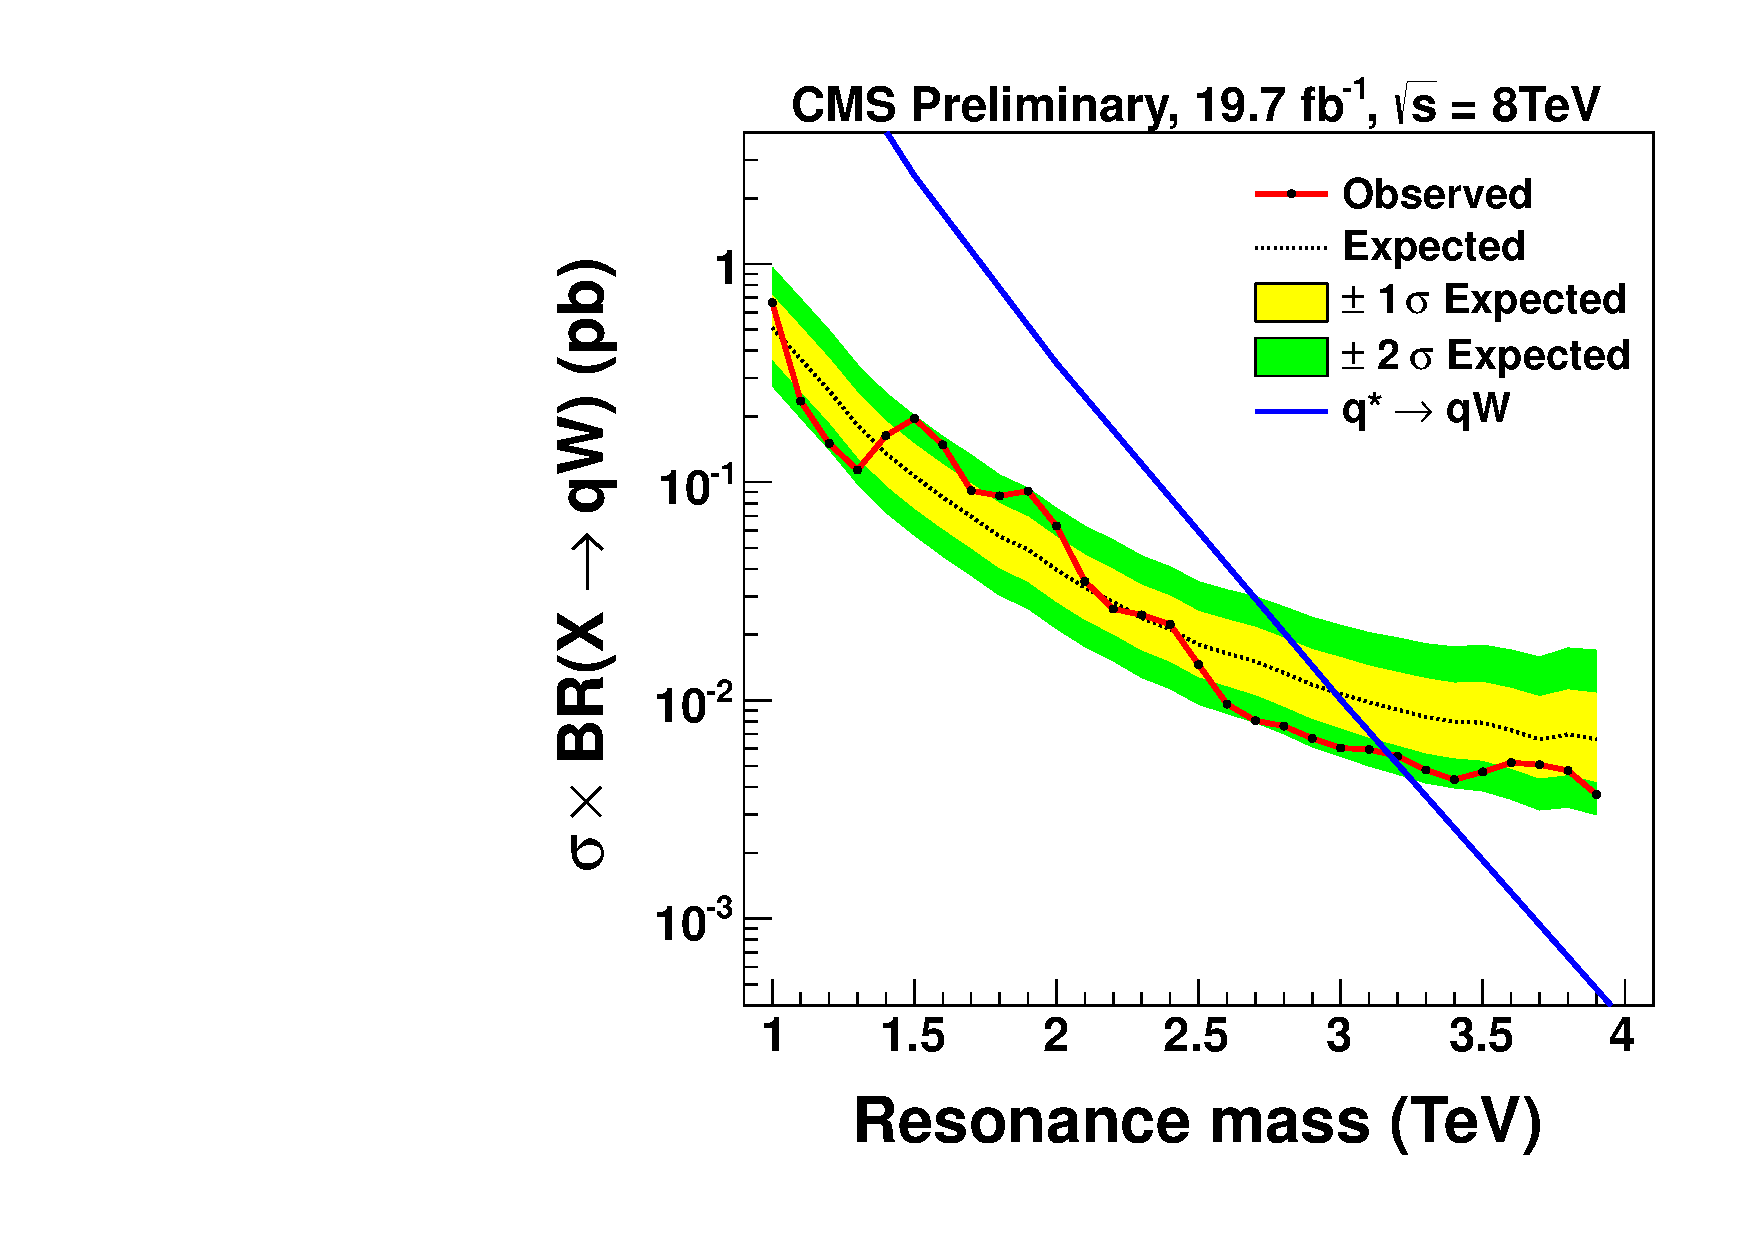
\includegraphics[width=0.49\textwidth]{EXO-12-024/figs/limits/brazilianFlag_qW_combined.pdf}
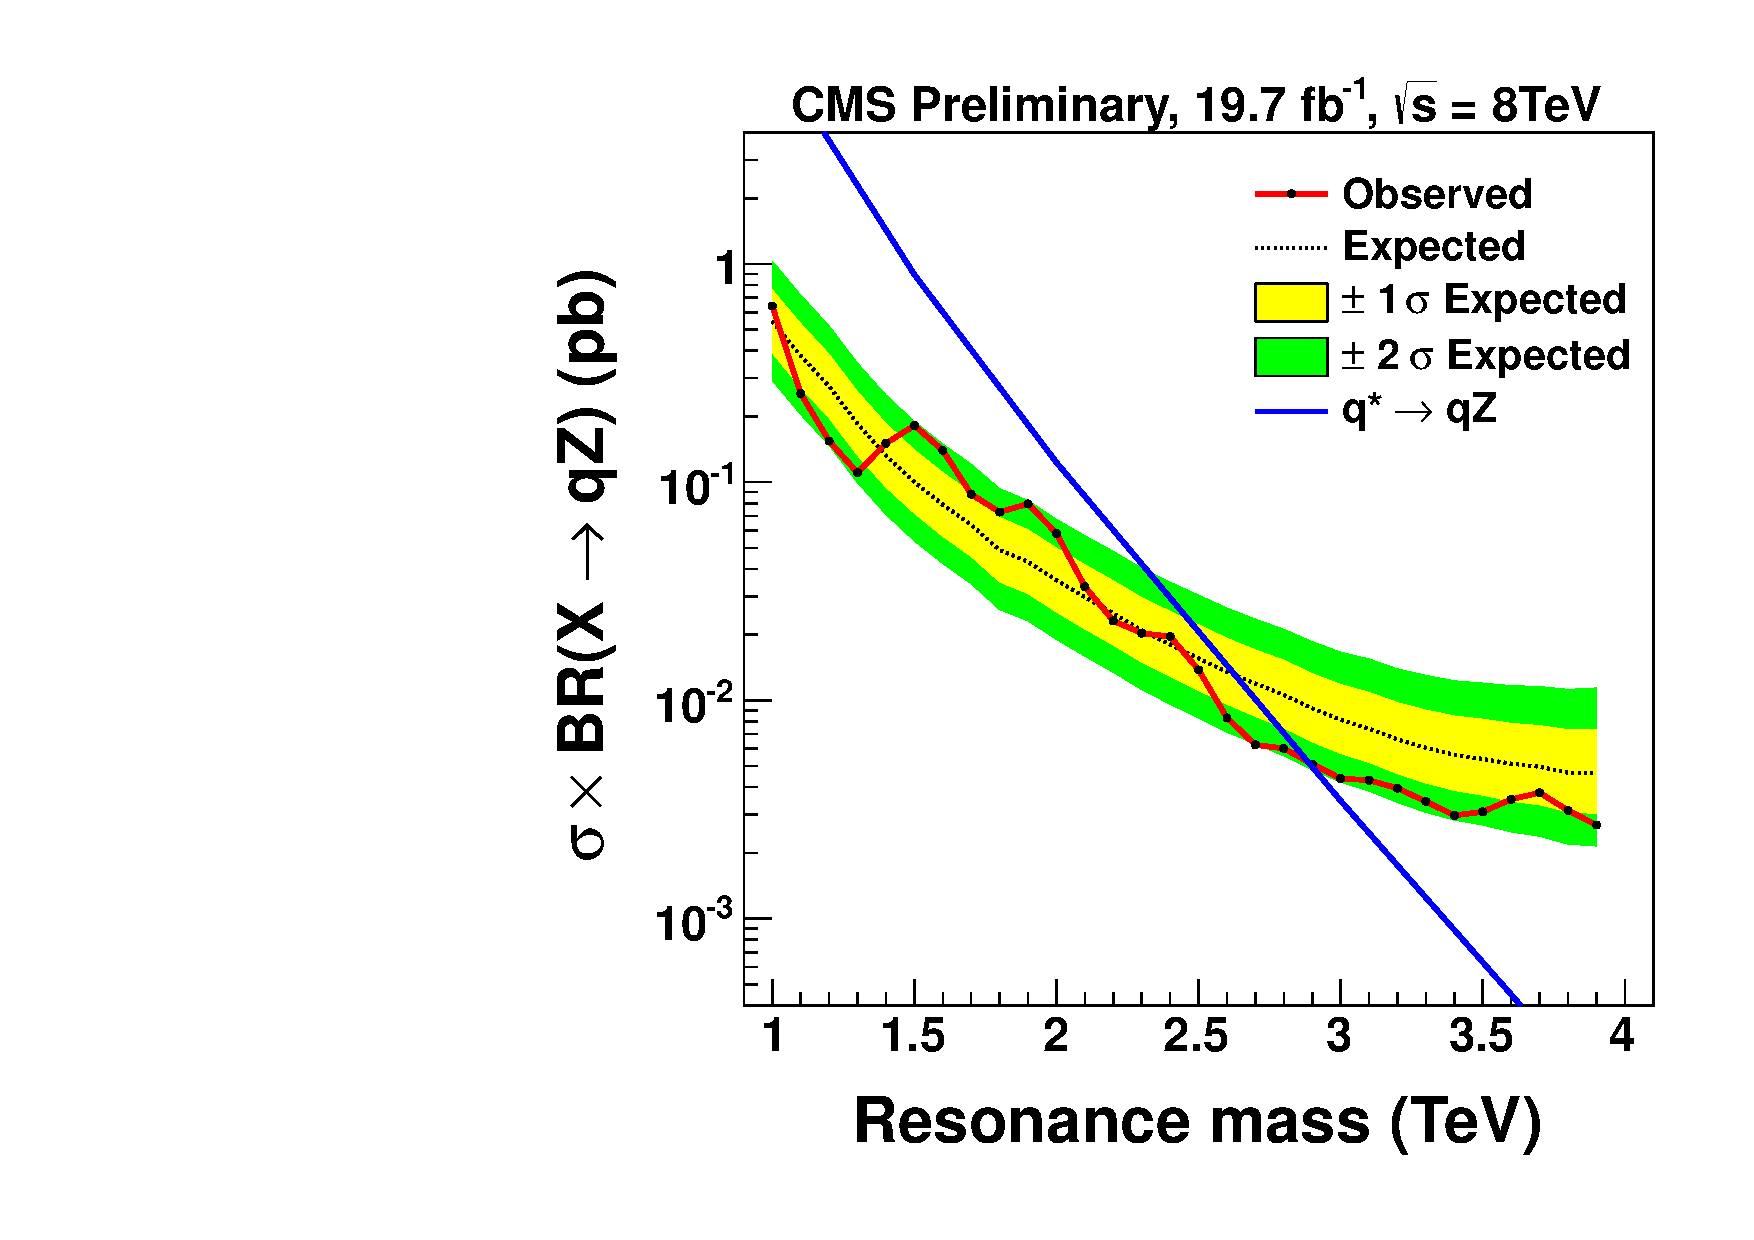
\includegraphics[width=0.49\textwidth]{EXO-12-024/figs/limits/brazilianFlag_qZ_combined.pdf}
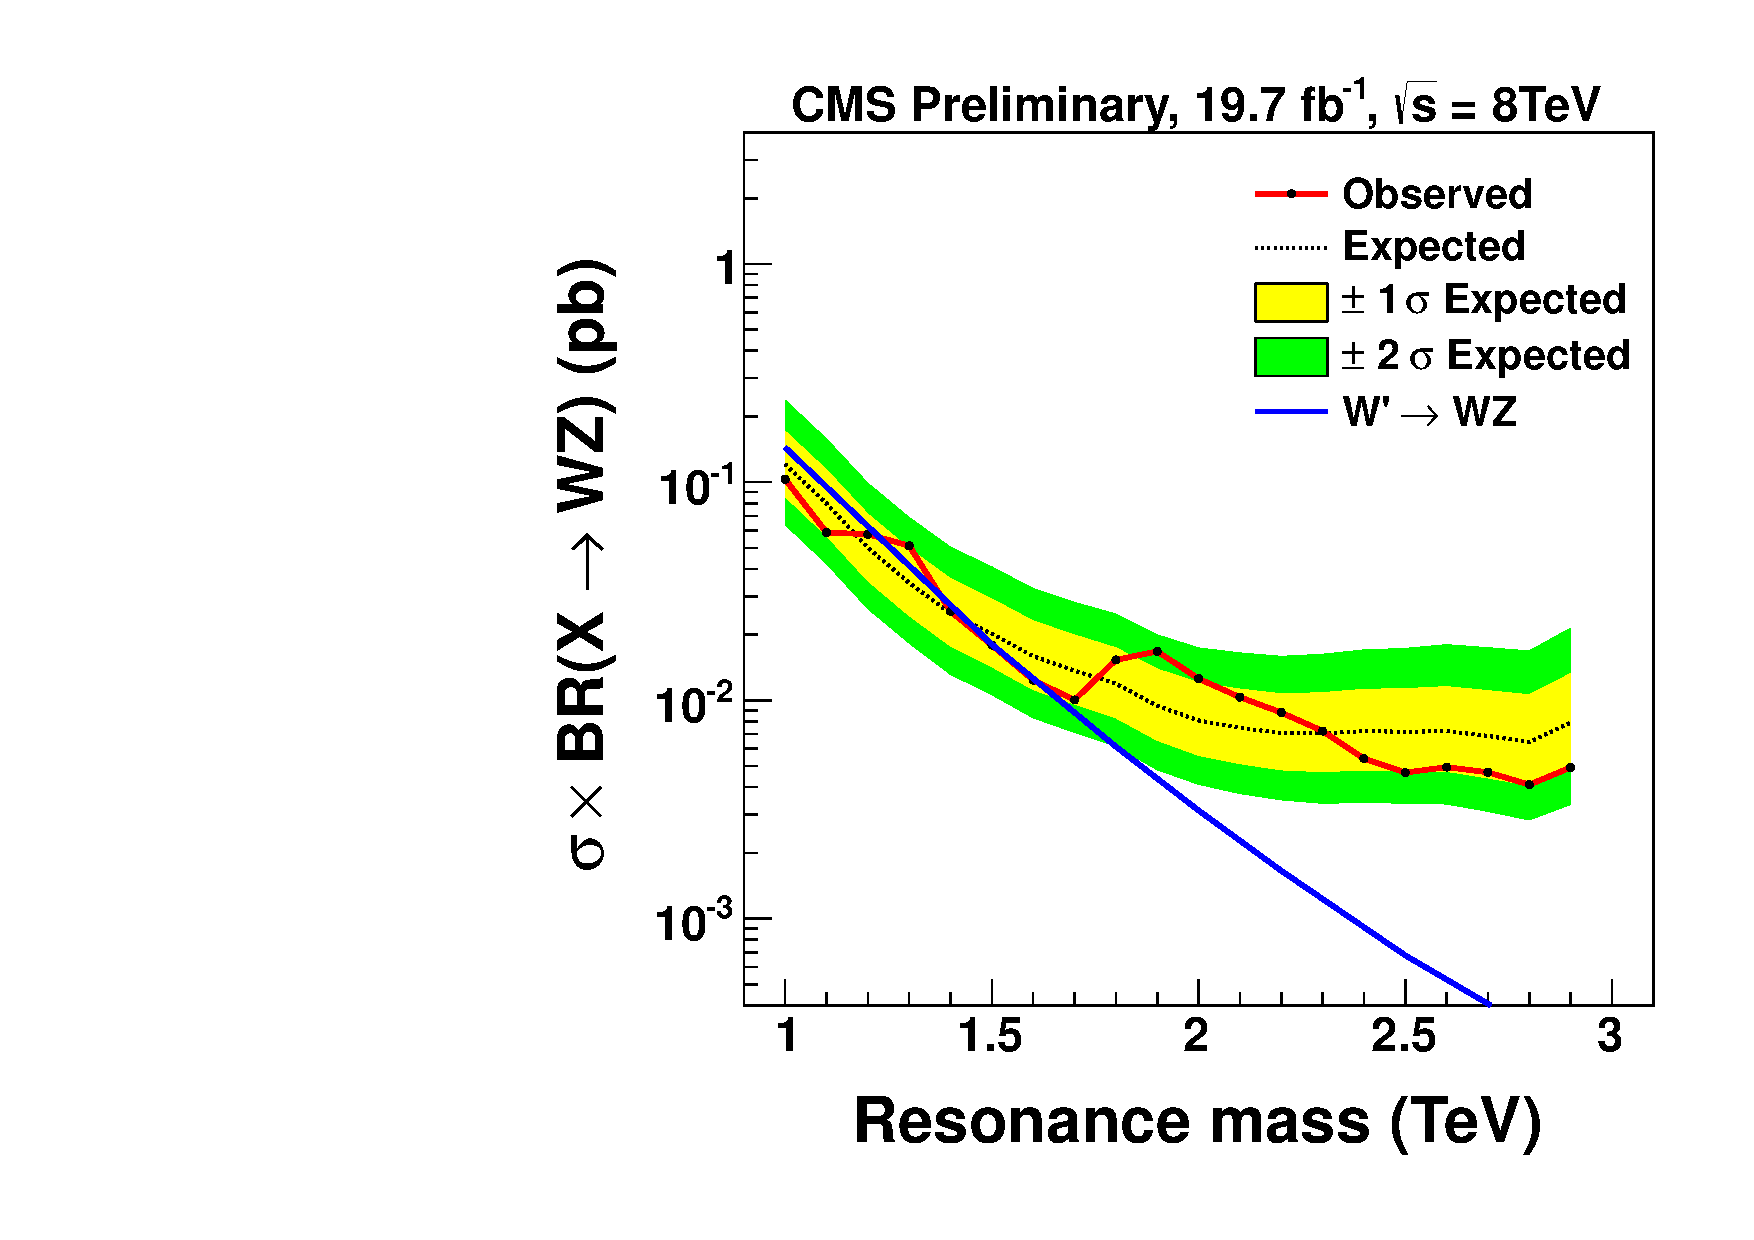
\includegraphics[width=0.49\textwidth]{EXO-12-024/figs/limits/brazilianFlag_WZ_combined.pdf}

\caption{Expected and observed 95\% CL limits on the production
  cross section as a function of the resonance mass for (upper left)
  qW resonances, (upper right) qZ resonances, and (bottom) WZ
  resonances, compared to their predicted cross sections for the
  corresponding benchmark models.}
\label{fig:Vtagresults}
\end{figure}

\begin{figure}[h!tb]
\centering
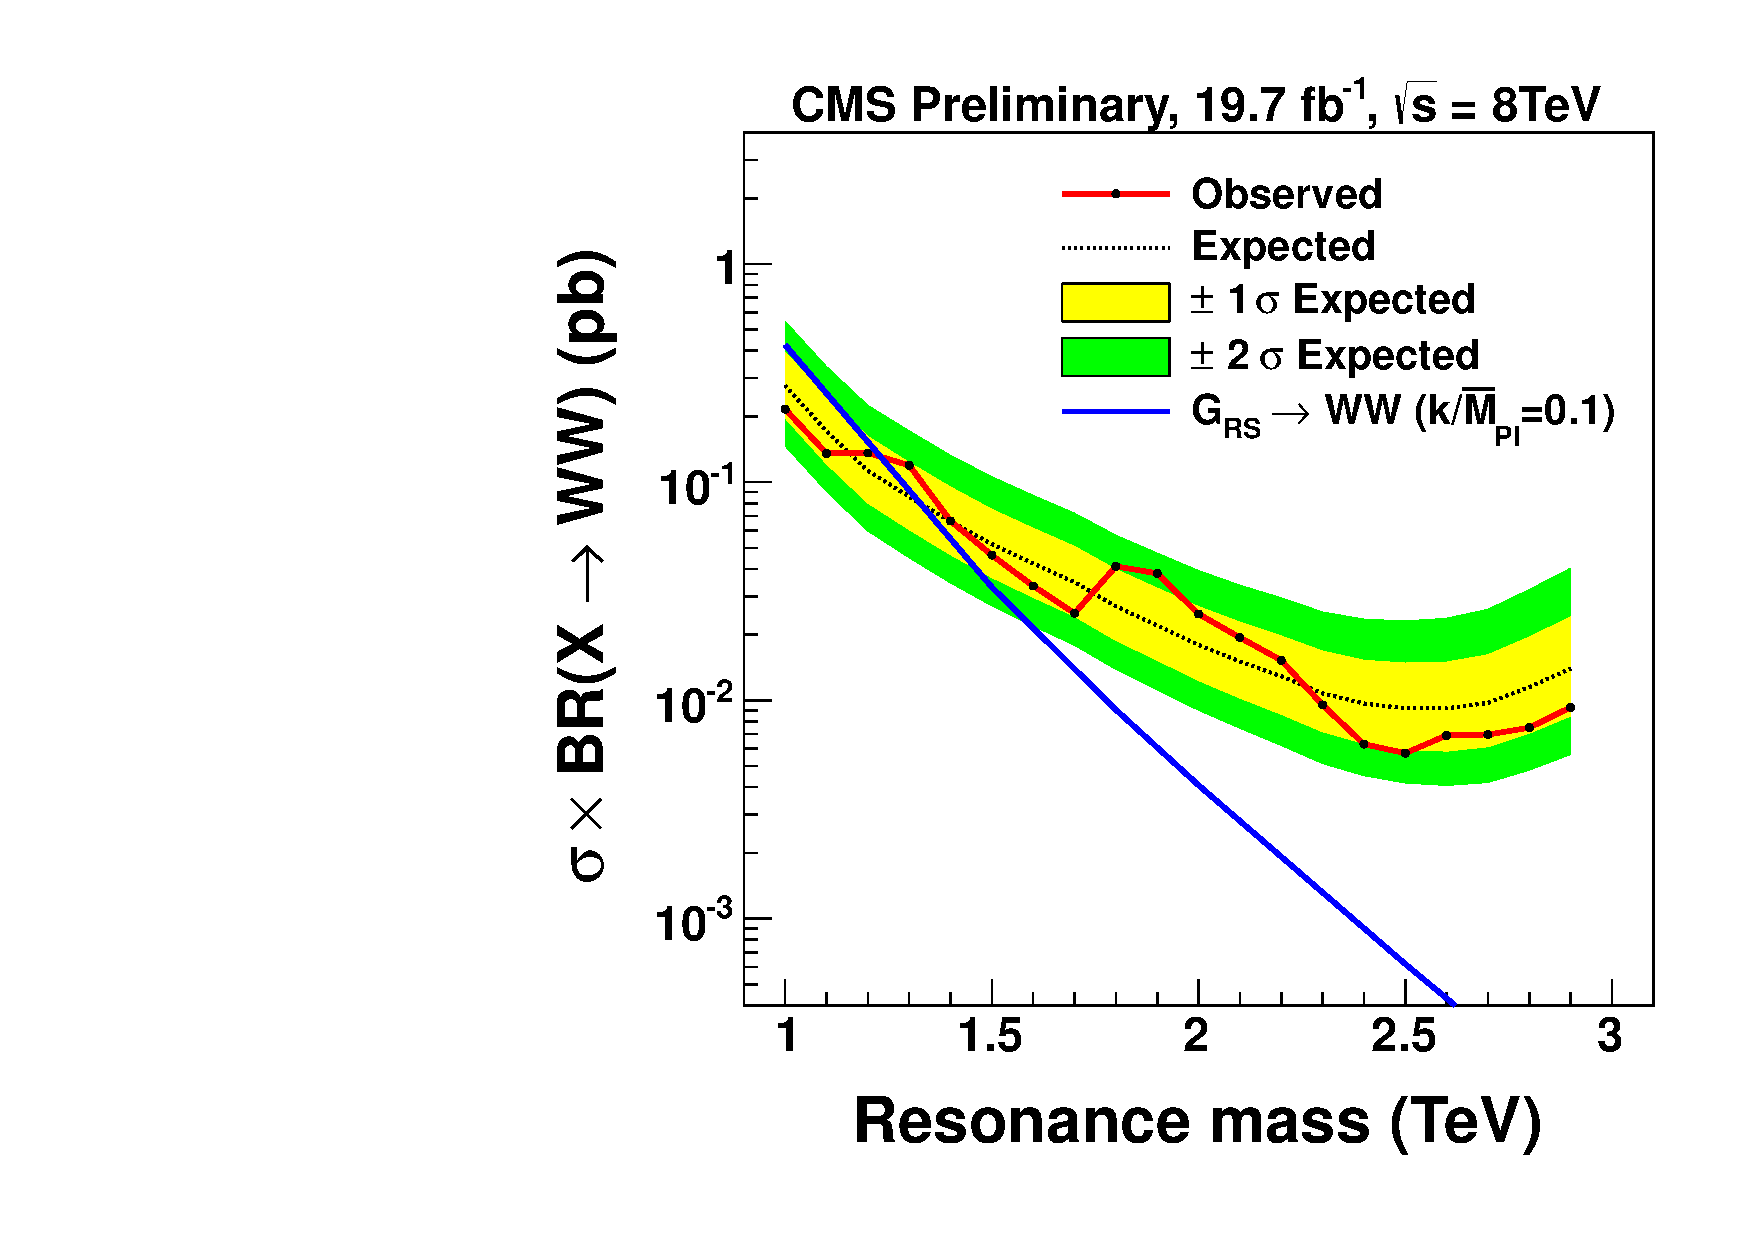
\includegraphics[width=0.49\textwidth]{EXO-12-024/figs/limits/brazilianFlag_RS1WW_combined.pdf}
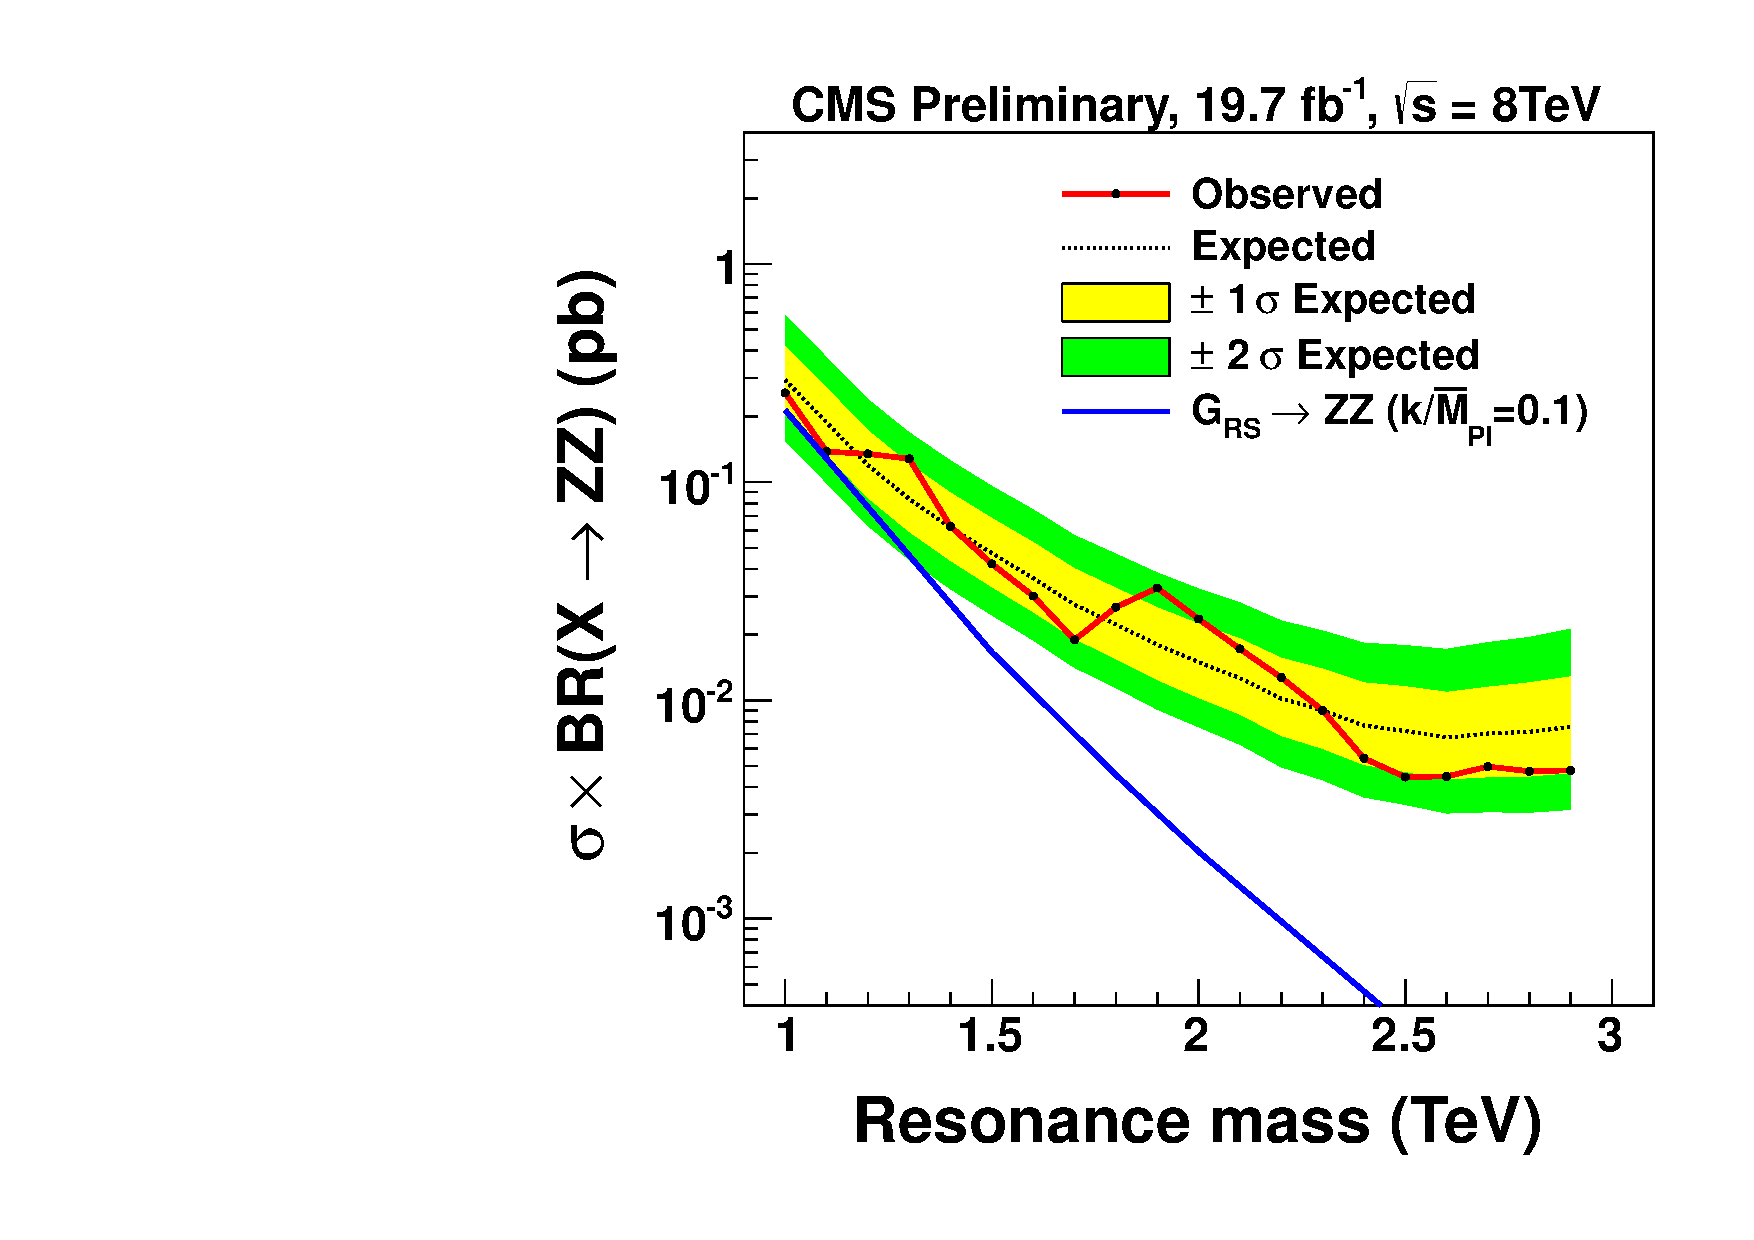
\includegraphics[width=0.49\textwidth]{EXO-12-024/figs/limits/brazilianFlag_RS1ZZ_combined.pdf}
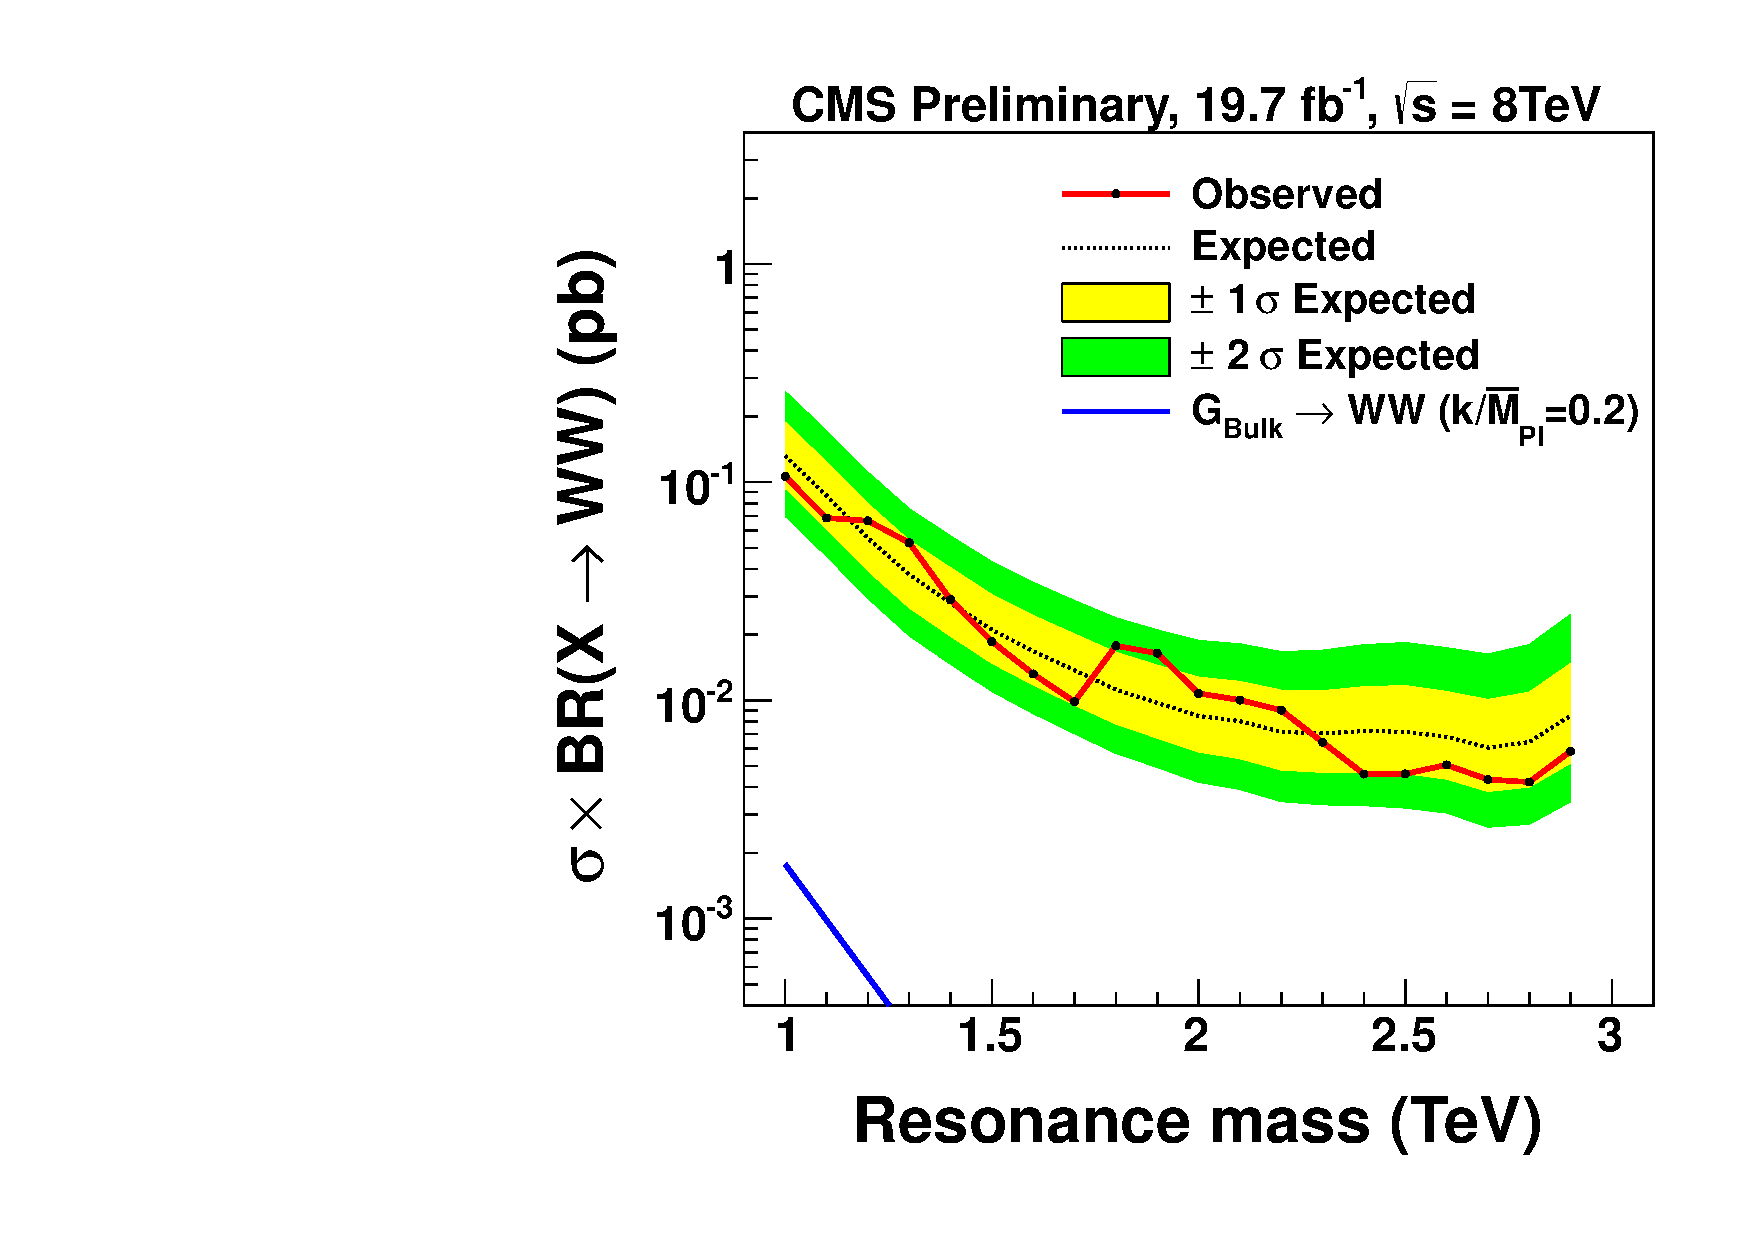
\includegraphics[width=0.49\textwidth]{EXO-12-024/figs/limits/brazilianFlag_BulkWW_combined.pdf}
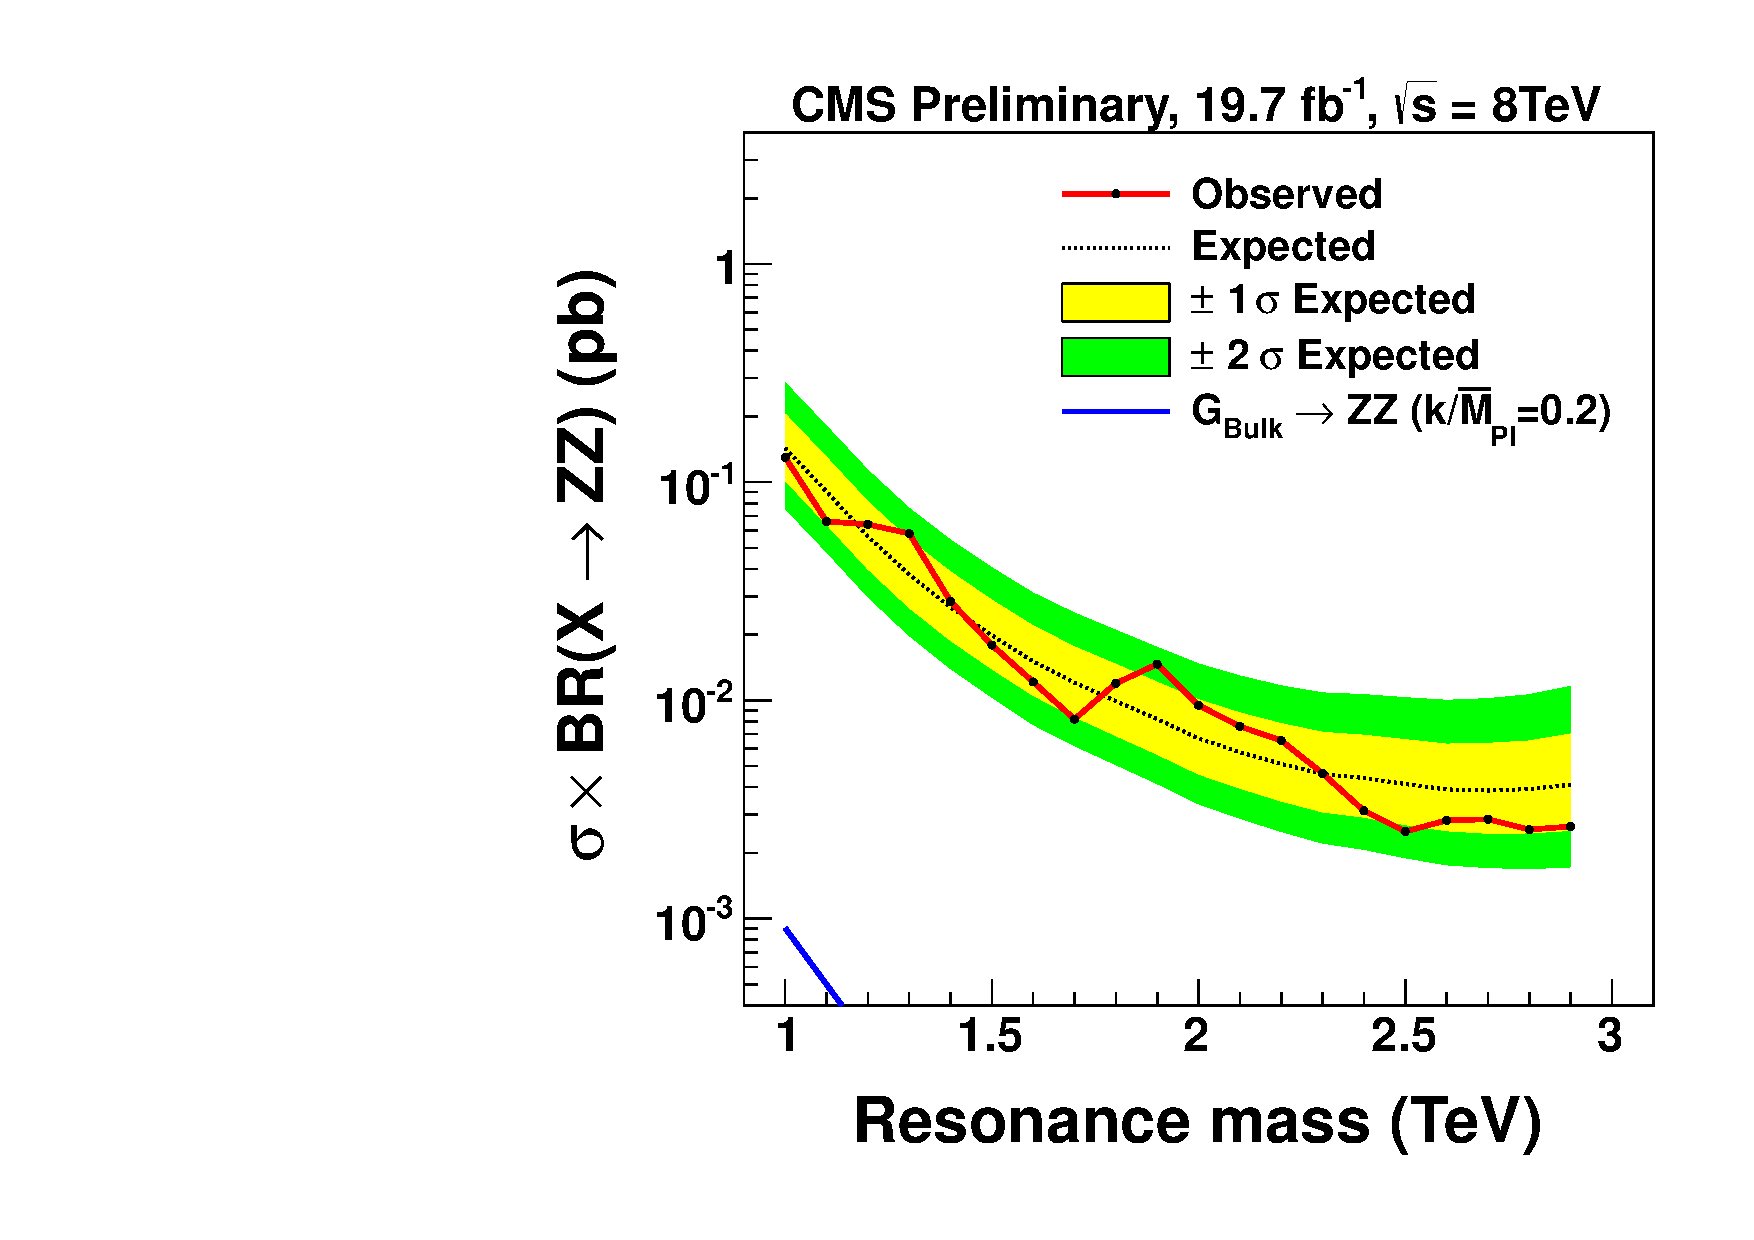
\includegraphics[width=0.49\textwidth]{EXO-12-024/figs/limits/brazilianFlag_BulkZZ_combined.pdf}
 \caption{Expected and observed 95\% CL limits on the production cross section
  as a function of the resonance mass for (upper left) \GRS$\to\PW \PW$ resonances,
  (upper right) \GRS$\to\cPZ \cPZ$ resonances, (bottom left) \GBulk$\to\PW \PW$ resonances, and
  (bottom right) \GBulk $\to\cPZ \cPZ$ resonances, compared to the predicted cross sections.
  \label{fig:Vtagresults2}}
\end{figure}

Figures~\ref{fig:Vtagresults} and~\ref{fig:Vtagresults2} show the
observed and background-only expected
upper limits on the production cross sections for singly and doubly
$\PW/\cPZ$-tagged events, computed at 95\% CL, with the predicted
cross sections for the benchmark models overlaid for
comparison. Table~\ref{table:results} shows the resulting exclusion
ranges on resonant masses. Compared to the previous search in this
channel at $\sqrt{s}=7$\TeVcc~\cite{ref_2011}, the mass limits on
$q*\to q\PW$ and $q*\to q\cPZ$ are increased, respectively,
by 0.8 and 0.7~\TeVcc and for the first time mass limits are set on
$\PWpr\to\PW\cPZ$ and \GRS$\to\PW \PW$ models. No mass limits are set
on \GRS$\to\cPZ \cPZ$, \GBulk$\to\PW \PW$ and \GBulk$\to\cPZ \cPZ$,
since the analysis is not sensitive to the small predicted cross
sections.

The systematic uncertainties have minor impact on the limits. The
largest contributions are 5\%, 5\%, and 3\% from $\PW/\cPZ$-tagging
efficiency, JES, and JER, respectively. These numbers are obtained by
quoting the largest change in the observed exclusion limit on the \GRS$
\to\PW\PW$ production cross section, over the entire examined mass
range, when the corresponding uncertainties are removed.

\begin{table}[htb]
\begin{center}
  \caption{Summary of observed limits on resonance masses at 95\% CL
    and their expected values, assuming a null
    hypothesis. The analysis is sensitive to resonances heavier than 1\TeVcc.\label{table:results}}
\begin{tabular}{ ccc}
\hline
Process      & Observed & Expected \\
& excluded mass limit (\TeVcc) & excluded mass limit (\TeVcc) \\
\hline
$q*\to q\PW $    & $3.2$  & $3.0$   \\
$q*\to q\cPZ $    & $2.9$  & $2.6$   \\
$\PWpr\to \PW\cPZ $  & $1.7$  & $1.6$   \\
\GRS$\to \PW \PW $  & $1.2$  & $1.3$   \\
\hline
\end{tabular}
\end{center}
\end{table}








\clearpage
